% Capítulo 4: pilha (LIFO) com empilhar e desempilhar no topo.
\documentclass[border=4pt]{standalone}
\usepackage[utf8]{inputenc}
\usepackage[T1]{fontenc}
% Estilo comum das figuras de listas (incluído pelas figuras dos capítulos 3 e 4).
\usepackage{tikz}
\usetikzlibrary{arrows.meta, positioning, shapes.multipart, calc}
\definecolor{navy}{RGB}{23,45,80}
\definecolor{laranja}{RGB}{250,110,29}
\definecolor{cinzalogo}{RGB}{107,114,126}
\tikzset{
  no/.style={rectangle split, rectangle split horizontal, rectangle split parts=2,
             draw=navy, line width=0.9pt, minimum height=7mm,
             rectangle split part fill={laranja!15, white}, font=\sffamily\small},
  no3/.style={rectangle split, rectangle split horizontal, rectangle split parts=3,
              draw=navy, line width=0.9pt, minimum height=7mm,
              rectangle split part fill={white, laranja!15, white}, font=\sffamily\small},
  seta/.style={-{Stealth[length=2.2mm]}, navy, line width=0.9pt},
  setanova/.style={-{Stealth[length=2.2mm]}, laranja, line width=1.3pt},
  rotulo/.style={font=\sffamily\small\bfseries, text=navy},
  nulo/.style={font=\sffamily\scriptsize, text=cinzalogo},
  passo/.style={font=\sffamily\small, text=cinzalogo, anchor=west},
  legenda/.style={font=\sffamily\scriptsize, text=cinzalogo},
}
% seta que sai do meio da caixa do ponteiro (última parte do nó), na horizontal
\newcommand{\liga}[3][seta]{\draw[#1] ([xshift=-2.3mm]#2.east) -- #3;}

\tikzset{caixa/.style={draw=navy, line width=0.9pt, minimum width=18mm, minimum height=7mm,
                        fill=laranja!12, font=\sffamily\small}}
\begin{document}
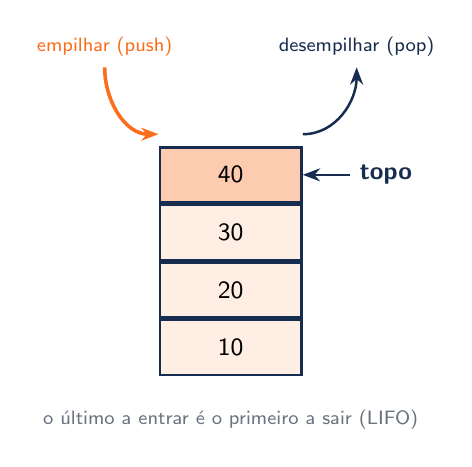
\begin{tikzpicture}
  \node[caixa] (c1) at (0,0) {10};
  \node[caixa, above=0mm of c1] (c2) {20};
  \node[caixa, above=0mm of c2] (c3) {30};
  \node[caixa, above=0mm of c3, fill=laranja!35] (c4) {40};
  \node[rotulo, right=6mm of c4] (topo) {topo};
  \draw[seta] (topo) -- (c4.east);
  \draw[setanova] ($(c4.north)+(-1.6,1.0)$) node[above, font=\sffamily\scriptsize, text=laranja] {empilhar (push)}
        to[out=-90, in=180] ($(c4.north west)+(0,0.15)$);
  \draw[seta] ($(c4.north east)+(0,0.15)$) to[out=0, in=-90]
        ($(c4.north)+(1.6,1.0)$) node[above, font=\sffamily\scriptsize, text=navy] {desempilhar (pop)};
  \node[legenda, below=3mm of c1] {o último a entrar é o primeiro a sair (LIFO)};
\end{tikzpicture}
\end{document}
